\documentclass[10pt,a4paper]{article}

% ---------- Codificación e idioma ----------
\usepackage[utf8]{inputenc}
\usepackage[T1]{fontenc}            % acentos y guiones bien en el PDF
\usepackage[english]{babel}
\DeclareUnicodeCharacter{2212}{-}   % el signo menos Unicode no rompe la compilación

% ---------- Página ----------
\usepackage[a4paper,margin=2cm]{geometry}   % 2 cm: límite de 2 páginas
\usepackage{microtype}              % mejor reparto de espacios, ahorra líneas

% ---------- Matemáticas ----------
\usepackage{amsmath,amssymb,amsthm}

% ---------- Unidades y química ----------
\usepackage{siunitx}
\sisetup{per-mode=symbol}           % kcal/mol en vez de kcal mol^-1
\DeclareSIUnit\calorie{cal}         % ¡usar \kilo\calorie, no \kilo\cal!
\DeclareSIUnit\atm{atm}
\DeclareSIUnit\hartree{\ensuremath{E_\mathrm{h}}}
\usepackage[version=4]{mhchem}

% ---------- Figuras y tablas ----------
\usepackage{graphicx}
\usepackage{booktabs}
\usepackage{float}
\usepackage[font=small,labelfont=bf]{caption}
\usepackage{tikz}
\usepackage{pgfplots}
\pgfplotsset{compat=1.18}

% ---------- Otros ----------
\usepackage[normalem]{ulem}         % normalem: \emph sigue siendo cursiva

% ---------- Compactación (para el límite de 2 páginas) ----------
\usepackage{titling}                % título más compacto
\setlength{\droptitle}{-1.6cm}
\pretitle{\begin{center}\large\bfseries}\posttitle{\par\end{center}\vspace{-0.6em}}
\preauthor{\begin{center}\normalsize}\postauthor{\par\end{center}\vspace{-0.9em}}
\predate{\begin{center}\small}\postdate{\par\end{center}\vspace{-1.2em}}
\usepackage{titlesec}               % secciones con menos espacio alrededor
\titleformat{\section}{\large\bfseries}{\thesection}{0.6em}{}
\titlespacing*{\section}{0pt}{1.1ex plus 0.3ex}{0.5ex}
\usepackage[shortlabels]{enumitem}  % listas sin espacios extra
\setlist{nosep, leftmargin=*}
\setlength{\intextsep}{6pt plus 2pt minus 2pt}       % espacio alrededor de figuras/tablas [H]
\captionsetup{skip=4pt}
\setlength{\parskip}{0pt}
\usepackage{etoolbox}               % bibliografía más pequeña y sin huecos
\apptocmd{\thebibliography}{\footnotesize\setlength{\itemsep}{0pt}\setlength{\parsep}{0pt}}{}{}

% ---------- Referencias (siempre al final y en este orden) ----------
\usepackage[hidelinks]{hyperref}
\usepackage[capitalise,noabbrev]{cleveref}



\title{From a double well to a single barrier:\\the \ce{S_N}2 reaction
\ce{F- + CH3Cl} in the gas phase and in water}
\author{Martín Llorens Giménez\thanks{\textbf{Declaration of AI use:} An AI assistant (Claude Opus 5.5, Anthropic) was used for guidance to help structure the text, which the author then wrote independently. AI was mainly used to revise English expressions and grammar, and to write the Python (matplotlib) code for figures and tables. All calculations, data extraction, and final decisions on the content are the author's own.}}
\date{November 2026}


\begin{document}

\maketitle

%Attention:
% - 2 pages maximum
% - Numbering of figures and tables, inclusion of figure/table captions
% - Units!
% - Use correct number of significant figures (we will discuss this)

\section{Introduction} %What have i done?

An \ce{S_N}2 reaction is a single, concerted step in which a nucleophile
attacks an sp\textsuperscript{3} carbon from the side opposite to the
leaving group while the bond to it breaks, so that the configuration is
inverted (Walden inversion)~\cite{Clayden2012}. By default, Gaussian
treats molecules as isolated, that is, in the gas phase. Under these
conditions, the ion and the molecule attract each other before reacting
and form ion--dipole complexes, and the reaction profile shows two
wells~\cite{Olmstead1977}. In solution, however, the \ce{S_N2} reaction
of \ce{F-} in a protic solvent such as water is known to be slow, since
\ce{F-} is strongly solvated~\cite{Clayden2012}.

The hypothesis of this work is that water, which stabilises ions more
strongly the more concentrated their charge is, will stabilise \ce{F-}
much more than the transition state (TS), where the charge is shared
between F and Cl. As a result, the ion--dipole complexes should
disappear and the TS should rise above the separated reactants: the
double well should turn into a barrier.

To test it, the potential energy surface (PES) of the reaction
\ce{F- + CH3Cl -> CH3F + Cl-} was computed (Exercise~3) and used to
locate the TS (Exercise~4, the exercise reported here). As an extension
beyond the exercise, the calculations were repeated with a continuum
solvent model (PCM, water), and the energy profiles, solvation energies
and rate constants in both media were compared.

\section{Methods} %How did i do it?

All calculations were performed with Gaussian~09~\cite{gaussian09} at the
HF/6-31+G* level. The diffuse functions (+) are required to describe the
extended electron density of the anions, and the polarisation functions (*) add
d functions on the heavy atoms. All species are closed-shell singlets. Reactants,
products and the two ion--dipole complexes were optimized and characterised by
harmonic frequency calculations.

The PES was obtained through a relaxed scan of $d$(C--F) from 1.3 to
\SI{2.9}{\angstrom} and $d$(C--Cl) from 3.6 to \SI{1.6}{\angstrom}, in steps of
\SI{0.2}{\angstrom} (99 points), optimizing all other coordinates at each point; a
dummy atom was used to define the collinear F--C--Cl arrangement without
\ang{180} angles. The TS search started from the saddle point of the scan
(\SI{2.2}{\angstrom}, \SI{2.1}{\angstrom}) with a planar \ce{CH3} group
(H--C--F = \ang{90}), using \texttt{opt=(ts,calcfc,noeigentest)}, and was
confirmed by a single imaginary frequency. Solvent effects were modelled with the
polarizable continuum model~\cite{Tomasi2005} (\texttt{scrf=(pcm,solvent=water)}),
re-optimizing all species and repeating the relaxed scan. Energies are given at
\SI{298.15}{\kelvin} and 1~atm (1~$E_\mathrm{h}$ = 627.51~kcal/mol). Rate constants
were obtained from transition state theory,
$k = (\frac{k_\mathrm{B}T}{h}) \cdot (\frac{RT}{P^\circ})^{n-1} \cdot e^{(-\Delta G^\ddagger/RT)}$,
where $n$ is the molecularity of the step.

\section{Results and discussion} %What are the results?


\textbf{Gas phase: a double well.} The gas-phase PES (\cref{fig:pes}a) shows two
closed valleys, which coincide with the independently optimized ion--dipole
complexes (RC and PC), and a saddle point between them. The scan energies reproduce
the reference data provided with the session, which validates the procedure. The
optimized TS has a single imaginary frequency (442$i$~cm$^{-1}$), whose normal
mode is the \ce{S_{N}2} itself: F approaches C, Cl leaves and the \ce{CH3}
umbrella inverts. Its geometry is collinear and almost symmetric
($d$(C--F) = \SI{2.125}{\angstrom}, $d$(C--Cl) = \SI{2.133}{\angstrom}), and matches
the saddle point of the scan to \SI{0.01}{\angstrom}. However, the H--C--F angle
(\ang{82.7}) is closer to the reactant complex (\ang{\sim 72}) than to the product
complex (\ang{\sim 109}): as expected from Hammond's postulate for a strongly
exergonic reaction, the TS is early and reactant-like.

\begin{figure}[H]
  \centering
  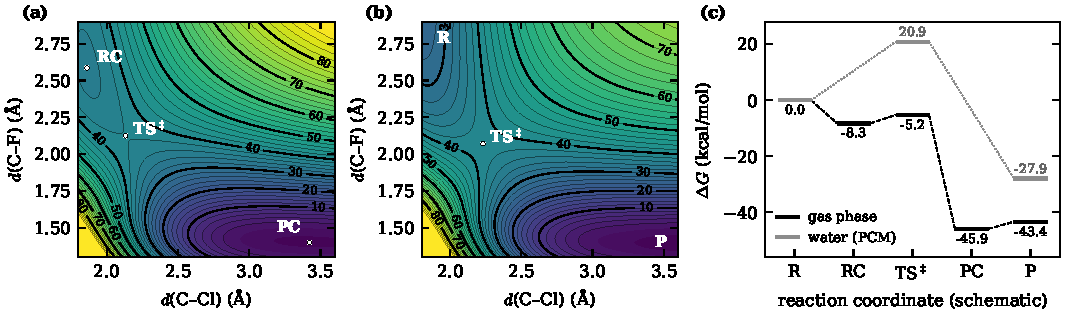
\includegraphics[scale=0.72]{figure1.pdf}
  \caption{PES of the reaction at the HF/6-31+G* level in (a) the gas phase and
    (b) water (PCM), from relaxed scans (energies relative to the lowest point of
    each scan; contours every 2~kcal/mol; $d$(C--Cl) $\geq$ \SI{1.8}{\angstrom}).
    RC, PC and TS$^\ddagger$ mark the optimized reactant complex, product complex and
    transition state; R and P, the reactant and product valleys. (c) Free-energy
    profiles relative to the separated reactants (R); RC and PC are not minima in water.}
  \label{fig:pes}
\end{figure}

The scan, however, only provides the shape of the surface. With a grid step of
\SI{0.2}{\angstrom}, it does not contain the exact stationary points: the lowest
point of the product valley, at (3.4, \SI{1.5}{\angstrom}), lies 3.1~kcal/mol above
the optimized product complex, whose C--F distance (\SI{1.40}{\angstrom}) falls
between two grid points. All the energies discussed below therefore come from full
optimizations of the minima and the TS, not from the scan.


\Cref{tab:profile} and \cref{fig:pes}c show the resulting profile. The reactant
complex lies 14.5~kcal/mol below the separated reactants ($\Delta E$), and the TS
only 3.0~kcal/mol above the complex, that is, 11.5~kcal/mol \emph{below} the
separated reactants: there is no net barrier, in agreement with the double-well
model~\cite{Olmstead1977}. In free energy, the TS rises to $-5.2$~kcal/mol, because
joining two particles into one lowers the entropy ($-T\Delta S \approx
+6$~kcal/mol). From the reactant complex ($\Delta G^\ddagger = 3.06$~kcal/mol,
$n = 1$), $k = 3.5\times10^{10}$~s$^{-1}$.

\begin{table}[H]
  \centering
  \caption{Energies relative to \ce{F- + CH3Cl} (kcal/mol) in the gas phase and in
    water (PCM).}
  \label{tab:profile}
  \footnotesize
  \begin{tabular}{l S[table-format=-2.2] S[table-format=-2.2] S[table-format=-2.2]
                    S[table-format=-2.2] S[table-format=-2.2]}
    \toprule
    & \multicolumn{3}{c}{Gas phase} & \multicolumn{2}{c}{Water (PCM)} \\
    \cmidrule(lr){2-4}\cmidrule(lr){5-6}
    Species & {$\Delta E$} & {$\Delta H$} & {$\Delta G$} & {$\Delta E$} & {$\Delta G$} \\
    \midrule
    \ce{F- + CH3Cl}        &   0.00 &   0.00 &   0.00 &   0.00 &   0.00 \\
    \ce{F-\bond{...}CH3Cl} & -14.51 & -14.39 &  -8.29 &  {--}  &  {--}  \\
    TS                     & -11.52 & -12.03 &  -5.22 &  14.03 &  20.86 \\
    \ce{FCH3\bond{...}Cl-} & -52.68 & -51.43 & -45.89 &  {--}  &  {--}  \\
    \ce{CH3F + Cl-}        & -44.64 & -43.64 & -43.37 & -29.13 & -27.88 \\
    \bottomrule
  \end{tabular}
\end{table}

\textbf{Water: a single barrier.} With PCM, neither complex survives: on
re-optimization, the ions move away to 4.5--\SI{5.1}{\angstrom}, where the surface is
flat, because the dielectric screens the ion--dipole attraction. In the water PES
(\cref{fig:pes}b), the closed wells of the gas phase become open valleys: the energy
keeps decreasing as either ion moves away. The TS, instead, remains a first-order
saddle point (547$i$~cm$^{-1}$, higher than in the gas phase: the barrier is not
only higher but also narrower) and now lies \emph{above} the reactants:
$\Delta G^\ddagger = 20.9$~kcal/mol, which gives
$k = 7.8\times10^{-2}$~M$^{-1}$\,s$^{-1}$ ($n = 2$). The double well has become a
single barrier, as predicted. The solvation energies, $E(\text{water}) -
E(\text{gas})$, explain why: $-86.2$~kcal/mol for \ce{F-}, $-70.5$ for \ce{Cl-} and
$-63.2$ for the TS (only $-2.5$ for \ce{CH3Cl}). The smaller the ion, the larger its
solvation, as in the Born model ($\propto -q^2/r$); in the TS, the charge is shared
between F and Cl. The reactants are therefore stabilised by 25.6~kcal/mol more than
the TS, which turns $-11.5$ into $+14.0$~kcal/mol. For the same reason
(\ce{F-} is better solvated than \ce{Cl-}), the reaction is less exergonic in water,
and the TS moves towards the products ($d$(C--F) = \SI{2.071}{\angstrom},
$d$(C--Cl) = \SI{2.231}{\angstrom}, H--C--F = \ang{86.0}), again as Hammond's
postulate predicts.


These results are qualitative. PCM only accounts for the dielectric constant of
water and does not include hydrogen bonds, which are especially strong for
\ce{F-}; the real solvation of \ce{F-} and the real barrier should therefore be even
larger. In addition, HF neglects electron correlation.

\section{Conclusion} %What can i conclude?

\begin{enumerate}
  \item In the gas phase, the \ce{S_{N}}2 reaction \ce{F- + CH3Cl} follows a
    double-well profile in which the TS (442$i$~cm$^{-1}$) lies 11.5~kcal/mol
    \emph{below} the separated reactants: there is no net barrier, and the only
    barrier, 3.1~kcal/mol in $\Delta G$, is the one from the reactant ion--dipole
    complex.
  \item Water (PCM) changes the profile completely: the ion--dipole complexes
    disappear and a barrier of 20.9~kcal/mol appears. This is because the solvent
    stabilises \ce{F-} ($-86.2$~kcal/mol), whose charge is concentrated, much more than
    the TS ($-63.2$~kcal/mol), where it is shared between F and Cl, as hypothesised.
    Hydrogen bonds, absent in PCM, would make the barrier even higher.
  \item As a consequence, the mechanism and the rate change: in the gas phase, the
    crossing of the TS is a unimolecular step from the complex,
    with $k = 3.5\times10^{10}$~s$^{-1}$, whereas in water it is a bimolecular
    reaction between the separated reactants, with
    $k = 7.8\times10^{-2}$~M$^{-1}$\,s$^{-1}$, which is slow at room temperature.
  \item The TS geometry is consistent with Hammond's postulate in both media: it is
    early and reactant-like in the gas phase (H--C--F = \ang{82.7}), and moves towards
    the products in water (\ang{86.0}), where the reaction is less exergonic.
\end{enumerate}
\bibliographystyle{unsrt}
\bibliography{bibliografia}

\end{document}
